%
% File emnlp2019.tex
%
%% Based on the style files for ACL 2019, which were
%% Based on the style files for EMNLP 2018, which were
%% Based on the style files for ACL 2018, which were
%% Based on the style files for ACL-2015, with some improvements
%%  taken from the NAACL-2016 style
%% Based on the style files for ACL-2014, which were, in turn,
%% based on ACL-2013, ACL-2012, ACL-2011, ACL-2010, ACL-IJCNLP-2009,
%% EACL-2009, IJCNLP-2008...
%% Based on the style files for EACL 2006 by 
%%e.agirre@ehu.es or Sergi.Balari@uab.es
%% and that of ACL 08 by Joakim Nivre and Noah Smith

\documentclass[11pt,a4paper]{article}
\usepackage[hyperref]{emnlp-ijcnlp-2019}
\usepackage{times}
\usepackage{latexsym}
\usepackage{graphicx}  %%% for including graphics
\usepackage{booktabs}


\usepackage{url}

%\aclfinalcopy % Uncomment this line for the final submission

%\setlength\titlebox{5cm}
% You can expand the titlebox if you need extra space
% to show all the authors. Please do not make the titlebox
% smaller than 5cm (the original size); we will check this
% in the camera-ready version and ask you to change it back.

\newcommand\BibTeX{B{\sc ib}\TeX}
\newcommand\confname{EMNLP-IJCNLP 2019}
\newcommand\conforg{SIGDAT}

\title{Instructions for \confname{} Proceedings}

\author{First Author \\
  Affiliation / Address line 1 \\
  Affiliation / Address line 2 \\
  Affiliation / Address line 3 \\
  {\tt email@domain} \\\And
  Second Author \\
  Affiliation / Address line 1 \\
  Affiliation / Address line 2 \\
  Affiliation / Address line 3 \\
  {\tt email@domain} \\}

\date{}

\begin{document}
\maketitle
\begin{abstract}
\end{abstract}


\newcommand{\refexp}[1]{\textsl{#1}}
\newcommand{\word}[1]{\textsl{#1}}
\newcommand{\cat}[1]{\textsc{#1}}
\newcommand{\vgenome}{VisualGenome\xspace}
\newcommand{\ra}{$\rightarrow$}

\newcommand{\sz}[1]{\textcolor{blue}{\emph{//sz: #1//}}}


\section{Introduction}

Expressions describing or referring to objects in visual scenes typically include a word naming the type of the object: e.g.,  \emph{cheesecake} or  \emph{dessert}  in Figure~\ref{fig:ex1}. 
Determining these objects names is a core aspect of virtually every language \& vision task, ranging from e.g.\ referring expression generation to visual dialogue.
Nevertheless, research in language \& vision has mostly  sidestepped questions about how speakers actually choose these names and how computational models should account for it.



While state-of-the-art computer vision systems are able to accurately classify images into thousands of different categories (e.g.\  \newcite{googlenet}), they mostly adopt very simple assumptions with respect to the underlying lexicon, which is typically implemented as a simple, flat labeling scheme. Thus, a standard object recognition system would be trained to classify the objects in Figure~\ref{fig:cake} as either  \emph{dessert} or \emph{cake}.
In contrast, humans seem to be more flexible as to the chosen level of generality and to the chosen part of the taxonomy (see objects in Figure \ref{fig:cake} that could be named \refexp{cake}, \refexp{cheesecake}, \refexp{dessert}, \refexp{sweet}, \refexp{pastry}, \refexp{food} etc.) 
Seminal work on prototypes suggests that the prototypicality of the object will determine the level of generality of the object name, i.e.\  a robin can be named \emph{bird}, but a penguin is better referred to as ``\emph{penguin}'' \cite{Rosch1978}.

%To date, surprisingly little work has been done on testing such theoretical predictions on large-scale, language \& vision data sets and integrating them explicitly into modeling frameworks.

\begin{figure}[htbp]
\begin{center}
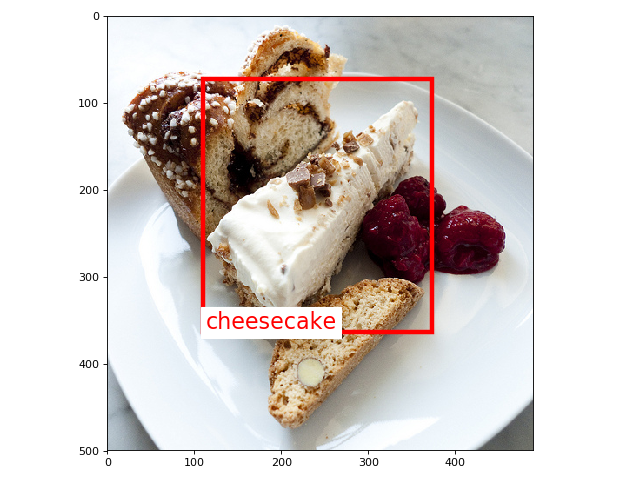
\includegraphics[height=3cm]{Figures/cheescake.png}
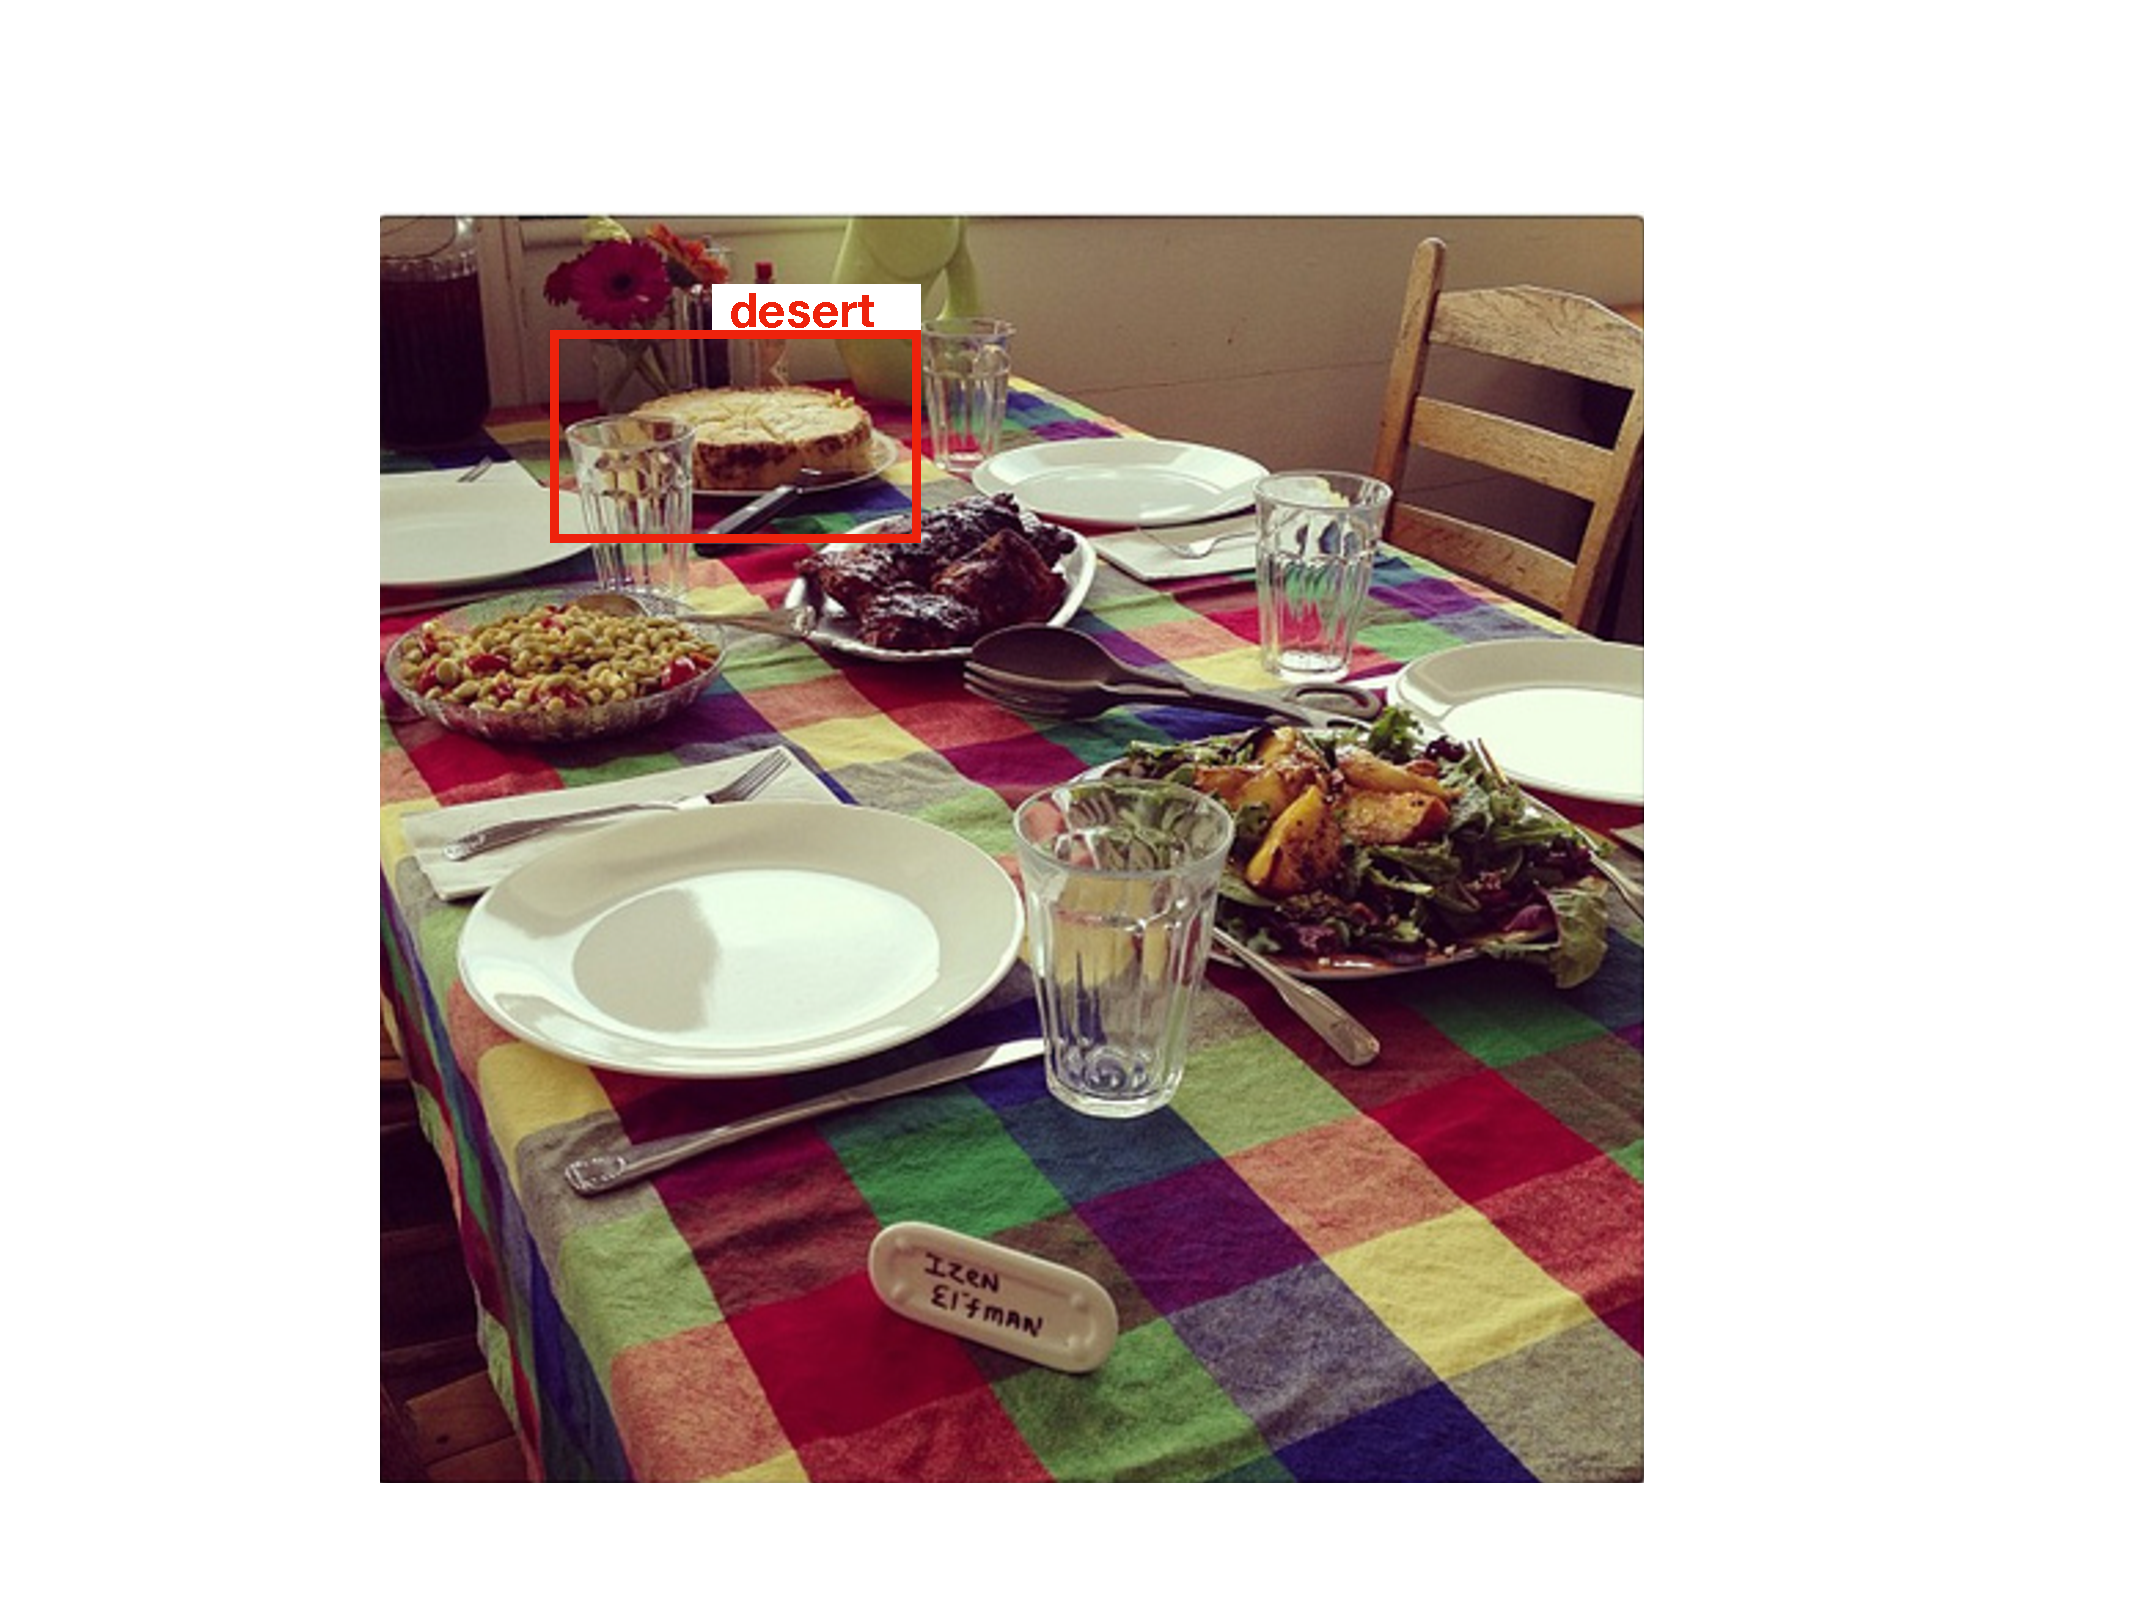
\includegraphics[height=3cm]{Figures/cheesecak2.pdf}
\caption{Two objects of the same type of cake, with different names in VisualGenome}
\label{fig:cake}
\end{center}
\end{figure}

\sz{something is missing here .. explain why exactly we did what we did, why is it interesting to collect many names for the same object?}

There are two main findings:

\begin{itemize}
\item the level of agreement in object naming is much higher in certain domains than in others, as it happens, the domains that have been traditionally used in object naming research (e.g. animals) seem to display the highest amount of agreement in our data set 
\item while previous work has mostly focussed on variation in the level of generality (\emph{penguin} vs. \emph{bird}), our datasets contains a lot of variability for names coming from different parts of the taxonomy (\emph{dessert} vs. \emph{cake}, \emph{bottle} vs. \emph{wine})
\end{itemize}


%The real-world objects that we interact with in our every-day life can be categorized into many thousands and maybe millions of categories. And even a single object can be member of many categories, i.e.\ at different taxonomical levels or in different parts of a taxonomy. For instance, both objects in Figure \ref{fig:cake} are at once instances of \cat{cake}, \cat{cheesecake}, \cat{dessert}, \cat{sweet}, \cat{pastry}, \cat{food} etc. Hence, when speakers name objects, e.g.\ when referring, they have to select a lexical item from a complex network of concepts and competing lexical alternatives.




%To date, research in NLP has surprisingly little to say about object naming, despite the fact that
% there has been a recent explosion of interest in various, and even complex, language \& vision tasks ranging from image captioning \cite{fangetal:2015,devlin:imcaqui,Bernardietal:automatic} to e.g.\ visual dialogue \cite{das2017visual,vries2017guesswhat}. 
%In contrast, closely related areas, such as computer vision and cognitive science, have investigated very related tasks in quite some depth: object recognition systems developed in the area of computer vision  are now able to classify images into thousands of different categories (e.g.\  \newcite{googlenet}).
%Furthermore, work on concepts, following the seminal work by Rosch, suggests that objects are typically conceptualized at a preferred level of specificity called the \textbf{entry-level}. Psycho-linguistic studies have been able to support this theory based on collections of so-called object naming norms. 
%
%This paper aims at addressing the genuinely linguistic questions revolving around the phenomenon of object naming by (i) presenting a collection of high-quality, large-scale naming data,  and (ii) analysis methods for this data and (iii) a first baseline model that accounts for the semantic flexibility of names for objects in real-world images. From computer vision, we borrow the idea of modeling realistic visual objects in realistic scenes (real-world images), but go beyond the simplistic assumption that object names correspond to unambiguous labels in a flat classification scheme (with no conceptual relations between the labels). From psycholinguistics, we borrow the idea of eliciting natural, representative naming data from many subjects, but go beyond using artificial, highly stylized objects.

\section{Related Work}

\section{Analysis}

\subsection{Agreement}

We compute the following agreement measures:

\begin{itemize}
\item \textbf{top \%}: for each object, we calculate the relative frequency of the most common name, and then average over all objects
\item \textbf{SD \%}: for each object, we calculate the Snodgrass agreement measure, and then average over all objects
\item \textbf{=VG}: the proportion of objects where the most frequent name coincides with the name annotated in VisualGenome
\end{itemize}


\begin{table*}
\small
\begin{tabular}{llll|llll|llll}
\toprule
    & \multicolumn{3}{c|}{all synsets} & \multicolumn{4}{c|}{max synset} & \multicolumn{4}{c}{min synset} \\
                         domain & \% top &    SD &   =VG &         id &     \% top &    SD &   =VG &             id &     \% top &    SD &   =VG \\
\midrule
                           person &  0.52 &  2.14 &  0.50 &  professional.n.01 &  0.61 &  2.02 &  0.20 &           athlete.n.01 &  0.34 &  2.67 &  0.36 \\
                        tableware &  0.52 &  1.92 &  0.40 &      crockery.n.01 &  0.52 &  1.92 &  0.40 &          crockery.n.01 &  0.52 &  1.92 &  0.40 \\
              clothing &  0.64 &  1.59 &  0.70 &      neckwear.n.01 &  0.79 &  0.91 &  0.77 &          footwear.n.01 &  0.47 &  2.55 &  0.40 \\
 instruments &  0.66 &  1.52 &  0.79 &    furnishing.n.02 &  0.67 &  1.50 &  0.80 &   kitchen\_utensil.n.01 &  0.60 &  1.85 &  0.56 \\
                solid food &  0.67 &  1.43 &  0.56 &   baked\_goods.n.01 &  0.67 &  1.43 &  0.56 &       baked\_goods.n.01 &  0.67 &  1.43 &  0.56 \\
          structure &  0.67 &  1.55 &  0.73 &        bridge.n.01 &  0.75 &  1.21 &  0.87 &  place\_of\_worship.n.01 &  0.46 &  2.26 &  0.08 \\
       %                       all &  0.70 &  1.35 &  0.73 &               None &  None &  None &  None &                   None &  None &  None &  None \\
                          vehicle &  0.72 &  1.13 &  0.71 &         train.n.01 &  0.93 &  0.43 &  0.99 &          aircraft.n.01 &  0.52 &  1.50 &  0.41 \\
                   food, nutrient &  0.72 &  1.27 &  0.68 &  edible\_fruit.n.01 &  0.80 &  0.89 &  0.79 &         vegetable.n.01 &  0.52 &  1.99 &  0.15 \\
         plants &  0.79 &  0.86 &  0.73 &        flower.n.01 &  0.79 &  0.86 &  0.73 &            flower.n.01 &  0.79 &  0.86 &  0.73 \\
                             ware &  0.82 &  0.96 &  0.94 &       cutlery.n.02 &  0.82 &  0.96 &  0.94 &           cutlery.n.02 &  0.82 &  0.96 &  0.94 \\
                             tool &  0.86 &  0.73 &  0.94 &          tool.n.01 &  0.86 &  0.73 &  0.94 &              tool.n.01 &  0.86 &  0.73 &  0.94 \\
                           animal &  0.91 &  0.43 &  0.94 &        feline.n.01 &  0.95 &  0.29 &  0.99 &              fish.n.01 &  0.39 &  2.53 &  0.55 \\
\bottomrule
 all &  0.70 &  1.35 &  0.73            \\

\bottomrule
\end{tabular}
\caption{Agreement in object names for objects of different domains, if applicable, synsets with maximal and minimal agreement (top \%) are shown }
\label{tab:agree}
\end{table*}

Table \ref{tab:agree} shows that, overall, our annotators achieve a fair amount of agreement in the object naming choices. The domain where annotators agree most is the animal domain, which, interestingly, happens to be the domain that has been mostly discussed in the object naming literature. \sz{... much more to say}

Why is naming more flexible in certain domains than in others?

\subsection{Lexical relations}

In this section, we take a closer look at the lexical variation we observe in our data set. We analyze the data points where participants attributed different names to the same object and extract a set of  pairwise \textbf{naming variants}. These naming variants correspond to pairs of words that can be used interchangeably to name certain objects.
For each object, we extract the set of naming variants $s = \{ (w_{top},w_2), (w_{top},w_3), (w_{top},w_4),... \}$  where $w_{top}$ is the most frequent name annotated for the object and $w_2 ... w_n$ constitute the less frequent alternatives of $w_{top}$.  The  \textbf{type frequency} of a naming variant $(w_{top},w_x)$ corresponds to the number of objects where this variant occurs. The \textbf{token frequency} of $(w_{top},w_x)$ corresponds the count of all annotations where $w_x$ has been used instead of $w_{top}$.
In Table \ref{tab:exvariants}, we show the the naming variants with the highest raw token frequency for each domain. \sz{domains need to be updated}


The naming variants can be grouped according to their lexical relation, as follows:

\begin{itemize}
\item \textbf{synonymy}: e.g.\ aircraft vs. airplane 
\item \textbf{hyponymy}: e.g.\ man vs. person
\item \textbf{co-hyponymy}: e.g.\ chicken vs. dinner, swan vs. goose
\item \textbf{no relation}: e.g.\  desk vs. apple
\end{itemize}


\begin{table}
\small
\begin{tabular}{llll}
\toprule
        relation & \% types & \% tokens & av. depth \\
\midrule
 co-hyponymy (closure, max depth=10) &  0.889 &  0.551 &       3.479 \\
    hyponymy (closure, max depth=10) &  0.097 &  0.328 &       2.204 \\
        synonymy &  0.015 &  0.121 &       1.000 \\
\bottomrule
\end{tabular}
\caption{Lexical relations between naming variants according to WordNet, for the set of name pairs where both words can be found in WordNet and stand in a \sz{should we produce this table for the different domains?}}
\label{tab:rel}
\end{table}


Research on object naming following the idea of entry-level categories has, essentially, exclusively looked at names that stand in a hierarchical relation (i.e.\ hyponymy/hypernymy).

We use WordNet to extract lexical relations between the naming variants in our data set.
Unfortunately, this means that we have to exclude a certain portion of the data as either (i) one of the name is not covered in WordNet, (ii) we cannot find a lexical relation between the two names (see below). Also, we had to be relatively permissive with respect to the definition of hyponymy/co-hyponymy. 
For instance, to analyze \textit{giraffe} as a hyponym of \textit{animal} we have to look at the closure of the hyponyms of \textit{animal} with a depth of 8 (in WordNet).
\sz{should we call this co-hyponymy or co-hierarchical relation?}

\sz{include Table that reports counts of the naming variants, coverage in WordNet etc.}

Table \ref{tab:rel} shows the distribution of lexical relations for those naming variants that we were able to analyze with WordNet.
Both in terms of their types and token frequency, the naming variants that instantiate a (loose) co-hyponymy relation are by far the most frequent.
\sz{discuss in more detail, discuss: to what extent is this an artefact of WordNet?}
This is really interesting: most research on object naming, to date, has focussed on hyponymy/hypernymy, i.e. variation that relates to hierarchical relations between object names.
Our data suggests that co-hierarchical variation is really important too.



\subsection{Issues with WordNet}



Some (interesting, somewhat cherry-picked) word pairs were WordNet does not find any relation (excluded in the above analysis):

\begin{itemize}
\item lettuce -- salad
\item fruit -- food
\item man -- catcher
\item bowl --chili
\item bowl -- diner
\item burger -- meat
\item statue -- animal (image shows statue of an animal)
\item bottle -- alcohol
\item donut --desert
\item zebra -- stripes
\item oven -- grill
\end{itemize}

\sz{discuss...}


\subsection{Entry-level names and preference orders....}

\sz{an interesting example:} In our data set, there are 24 images where \textit{penguin} has been used, so we know that the object is a \textit{penguin}. For 50\% of these images, annotators still prefer \textit{bird} as the most common name. According to the theory of entry-level categories, this should not happen. People should always prefer \textit{penguin} over \textit{bird}. 

\sz{how can we analyze this quantitatively?}

\begin{table*}
\small
\begin{tabular}{lp{12cm}}
\toprule
                         category &                                                                                                                                                                                                                    most frequent naming variants \\
\midrule
 food, solid food &  sandwich -- food (492), hotdog -- food (467), hotdog -- sandwich (318), cake -- food (265), bread -- sandwich (257), bread -- food (247), bread -- bun (206), donut -- food (188), hotdog -- bun (184), sandwich -- burger (163) \\
 structure, construction &  house -- building (1160), building -- house (511), bridge -- train (326), bridge -- overpass (235), house -- window (161), house -- home (123), tent -- canopy (120), building -- castle (101), bridge -- building (98), bridge -- pole (85) \\
 tool &  knife -- pizza (27), knife -- food (22), knife -- cake (17), knife -- banana (16), knife -- plate (15), knife -- apple (13), knife -- pocket knife (12), knife -- butter knife (12), knife -- table (10), knife -- carrot (8) \\
 vehicle &  airplane -- plane (11194), plane -- airplane (3829), motorcycle -- bike (2624), airplane -- jet (1319), boat -- ship (1301), truck -- car (1095), car -- vehicle (874), motorcycle -- wheel (861), truck -- vehicle (718), truck -- wheel (716) \\
 plant, flora, plant life &  flower -- flowers (29), rose -- flower (25), flower -- rose (22), flower -- vase (18), flowers -- flower (14), flower -- dandelion (14), plant -- flower (12), flower -- sunflower (11), plant -- wheat (11), flower -- flower pot (10) \\
 food, nutrient &  pizza -- food (1796), sandwich -- food (631), pizza -- cheese (447), pizza -- plate (423), salad -- food (402), sandwich -- burger (235), pizza -- toppings (217), pizza -- pizza slice (162), sandwich -- bread (156), food -- sandwich (147) \\
 tableware &  cup -- mug (146), mug -- cup (104), cup -- coffee (93), cup -- drink (73), bowl -- food (60), cup -- glass (39), bowl -- cup (36), glass -- wine glass (35), glass -- cup (34), cup -- coffee cup (31) \\
 article of clothing &  shirt -- t-shirt (2914), jacket -- coat (2396), jacket -- shirt (1552), jacket -- suit (1168), suit -- jacket (1029), shirt -- jacket (813), shirt -- tie (723), shirt -- man (487), shirt -- dress (462), shirt -- sweater (450) \\
 animal &  cow -- bull (515), sheep -- goat (486), cow -- animal (445), giraffe -- animal (380), bird -- parrot (349), sheep -- animal (294), sheep -- lamb (282), horse -- animal (269), cat -- animal (237), bird -- seagull (231) \\
 ware &  fork -- spoon (71), fork -- plate (44), spoon -- food (32), fork -- food (31), fork -- cake (21), spoon -- fork (18), spoon -- wooden spoon (15), fork -- broccoli (15), fork -- silverware (10), spoon -- vegetables (8) \\
 person &  woman -- person (3594), man -- person (3546), boy -- child (3243), woman -- girl (2328), girl -- child (1985), woman -- tennis player (1277), man -- player (1273), man -- boy (1214), skateboarder -- skater (1194), man -- t-shirt (1143) \\
 instrumentality, instrumentation &  couch -- sofa (4090), desk -- table (3435), carpet -- floor (1697), bench -- chair (1401), desk -- keyboard (1380), counter -- table (1201), table -- desk (1135), counter -- countertop (1101), table -- counter (906), rug -- carpet (895) \\
\bottomrule
\end{tabular}\caption{Most frequent naming variants for each category}
\label{tab:exvariants}
\end{table*}


\subsection{Co-hyponyms as names for objects}

\sz{analyze and discuss why we find so many co-hyponyms in our data set}

\section{Modeling}

\sz{I think, the prevalence of co-hyponymy is the most interesting finding. Can we learn to predict whether to co-hyponyms can be used to name the same object?}

\end{document}
